% Options for packages loaded elsewhere
\PassOptionsToPackage{unicode}{hyperref}
\PassOptionsToPackage{hyphens}{url}
%
\documentclass[
]{article}
\usepackage{amsmath,amssymb}
\usepackage{lmodern}
\usepackage{iftex}
\ifPDFTeX
  \usepackage[T1]{fontenc}
  \usepackage[utf8]{inputenc}
  \usepackage{textcomp} % provide euro and other symbols
\else % if luatex or xetex
  \usepackage{unicode-math}
  \defaultfontfeatures{Scale=MatchLowercase}
  \defaultfontfeatures[\rmfamily]{Ligatures=TeX,Scale=1}
\fi
% Use upquote if available, for straight quotes in verbatim environments
\IfFileExists{upquote.sty}{\usepackage{upquote}}{}
\IfFileExists{microtype.sty}{% use microtype if available
  \usepackage[]{microtype}
  \UseMicrotypeSet[protrusion]{basicmath} % disable protrusion for tt fonts
}{}
\makeatletter
\@ifundefined{KOMAClassName}{% if non-KOMA class
  \IfFileExists{parskip.sty}{%
    \usepackage{parskip}
  }{% else
    \setlength{\parindent}{0pt}
    \setlength{\parskip}{6pt plus 2pt minus 1pt}}
}{% if KOMA class
  \KOMAoptions{parskip=half}}
\makeatother
\usepackage{xcolor}
\usepackage[margin=1in]{geometry}
\usepackage{color}
\usepackage{fancyvrb}
\newcommand{\VerbBar}{|}
\newcommand{\VERB}{\Verb[commandchars=\\\{\}]}
\DefineVerbatimEnvironment{Highlighting}{Verbatim}{commandchars=\\\{\}}
% Add ',fontsize=\small' for more characters per line
\usepackage{framed}
\definecolor{shadecolor}{RGB}{248,248,248}
\newenvironment{Shaded}{\begin{snugshade}}{\end{snugshade}}
\newcommand{\AlertTok}[1]{\textcolor[rgb]{0.94,0.16,0.16}{#1}}
\newcommand{\AnnotationTok}[1]{\textcolor[rgb]{0.56,0.35,0.01}{\textbf{\textit{#1}}}}
\newcommand{\AttributeTok}[1]{\textcolor[rgb]{0.77,0.63,0.00}{#1}}
\newcommand{\BaseNTok}[1]{\textcolor[rgb]{0.00,0.00,0.81}{#1}}
\newcommand{\BuiltInTok}[1]{#1}
\newcommand{\CharTok}[1]{\textcolor[rgb]{0.31,0.60,0.02}{#1}}
\newcommand{\CommentTok}[1]{\textcolor[rgb]{0.56,0.35,0.01}{\textit{#1}}}
\newcommand{\CommentVarTok}[1]{\textcolor[rgb]{0.56,0.35,0.01}{\textbf{\textit{#1}}}}
\newcommand{\ConstantTok}[1]{\textcolor[rgb]{0.00,0.00,0.00}{#1}}
\newcommand{\ControlFlowTok}[1]{\textcolor[rgb]{0.13,0.29,0.53}{\textbf{#1}}}
\newcommand{\DataTypeTok}[1]{\textcolor[rgb]{0.13,0.29,0.53}{#1}}
\newcommand{\DecValTok}[1]{\textcolor[rgb]{0.00,0.00,0.81}{#1}}
\newcommand{\DocumentationTok}[1]{\textcolor[rgb]{0.56,0.35,0.01}{\textbf{\textit{#1}}}}
\newcommand{\ErrorTok}[1]{\textcolor[rgb]{0.64,0.00,0.00}{\textbf{#1}}}
\newcommand{\ExtensionTok}[1]{#1}
\newcommand{\FloatTok}[1]{\textcolor[rgb]{0.00,0.00,0.81}{#1}}
\newcommand{\FunctionTok}[1]{\textcolor[rgb]{0.00,0.00,0.00}{#1}}
\newcommand{\ImportTok}[1]{#1}
\newcommand{\InformationTok}[1]{\textcolor[rgb]{0.56,0.35,0.01}{\textbf{\textit{#1}}}}
\newcommand{\KeywordTok}[1]{\textcolor[rgb]{0.13,0.29,0.53}{\textbf{#1}}}
\newcommand{\NormalTok}[1]{#1}
\newcommand{\OperatorTok}[1]{\textcolor[rgb]{0.81,0.36,0.00}{\textbf{#1}}}
\newcommand{\OtherTok}[1]{\textcolor[rgb]{0.56,0.35,0.01}{#1}}
\newcommand{\PreprocessorTok}[1]{\textcolor[rgb]{0.56,0.35,0.01}{\textit{#1}}}
\newcommand{\RegionMarkerTok}[1]{#1}
\newcommand{\SpecialCharTok}[1]{\textcolor[rgb]{0.00,0.00,0.00}{#1}}
\newcommand{\SpecialStringTok}[1]{\textcolor[rgb]{0.31,0.60,0.02}{#1}}
\newcommand{\StringTok}[1]{\textcolor[rgb]{0.31,0.60,0.02}{#1}}
\newcommand{\VariableTok}[1]{\textcolor[rgb]{0.00,0.00,0.00}{#1}}
\newcommand{\VerbatimStringTok}[1]{\textcolor[rgb]{0.31,0.60,0.02}{#1}}
\newcommand{\WarningTok}[1]{\textcolor[rgb]{0.56,0.35,0.01}{\textbf{\textit{#1}}}}
\usepackage{graphicx}
\makeatletter
\def\maxwidth{\ifdim\Gin@nat@width>\linewidth\linewidth\else\Gin@nat@width\fi}
\def\maxheight{\ifdim\Gin@nat@height>\textheight\textheight\else\Gin@nat@height\fi}
\makeatother
% Scale images if necessary, so that they will not overflow the page
% margins by default, and it is still possible to overwrite the defaults
% using explicit options in \includegraphics[width, height, ...]{}
\setkeys{Gin}{width=\maxwidth,height=\maxheight,keepaspectratio}
% Set default figure placement to htbp
\makeatletter
\def\fps@figure{htbp}
\makeatother
\setlength{\emergencystretch}{3em} % prevent overfull lines
\providecommand{\tightlist}{%
  \setlength{\itemsep}{0pt}\setlength{\parskip}{0pt}}
\setcounter{secnumdepth}{5}
\ifLuaTeX
  \usepackage{selnolig}  % disable illegal ligatures
\fi
\IfFileExists{bookmark.sty}{\usepackage{bookmark}}{\usepackage{hyperref}}
\IfFileExists{xurl.sty}{\usepackage{xurl}}{} % add URL line breaks if available
\urlstyle{same} % disable monospaced font for URLs
\hypersetup{
  pdftitle={Repaso Faraway},
  pdfauthor={Felipe Yebes},
  hidelinks,
  pdfcreator={LaTeX via pandoc}}

\title{Repaso Faraway}
\author{Felipe Yebes}
\date{2023-10-01}

\begin{document}
\maketitle

{
\setcounter{tocdepth}{2}
\tableofcontents
}
\hypertarget{ejercicio-1}{%
\subsection{Ejercicio 1}\label{ejercicio-1}}

\begin{Shaded}
\begin{Highlighting}[]
\FunctionTok{data}\NormalTok{(pima, }\AttributeTok{package=}\StringTok{"faraway"}\NormalTok{)}
\FunctionTok{head}\NormalTok{(pima)}
\end{Highlighting}
\end{Shaded}

\begin{verbatim}
##   pregnant glucose diastolic triceps insulin  bmi diabetes age test
## 1        6     148        72      35       0 33.6    0.627  50    1
## 2        1      85        66      29       0 26.6    0.351  31    0
## 3        8     183        64       0       0 23.3    0.672  32    1
## 4        1      89        66      23      94 28.1    0.167  21    0
## 5        0     137        40      35     168 43.1    2.288  33    1
## 6        5     116        74       0       0 25.6    0.201  30    0
\end{verbatim}

\begin{Shaded}
\begin{Highlighting}[]
\CommentTok{\#Resumen\#}
\FunctionTok{summary}\NormalTok{(pima)}
\end{Highlighting}
\end{Shaded}

\begin{verbatim}
##     pregnant         glucose        diastolic         triceps     
##  Min.   : 0.000   Min.   :  0.0   Min.   :  0.00   Min.   : 0.00  
##  1st Qu.: 1.000   1st Qu.: 99.0   1st Qu.: 62.00   1st Qu.: 0.00  
##  Median : 3.000   Median :117.0   Median : 72.00   Median :23.00  
##  Mean   : 3.845   Mean   :120.9   Mean   : 69.11   Mean   :20.54  
##  3rd Qu.: 6.000   3rd Qu.:140.2   3rd Qu.: 80.00   3rd Qu.:32.00  
##  Max.   :17.000   Max.   :199.0   Max.   :122.00   Max.   :99.00  
##     insulin           bmi           diabetes           age       
##  Min.   :  0.0   Min.   : 0.00   Min.   :0.0780   Min.   :21.00  
##  1st Qu.:  0.0   1st Qu.:27.30   1st Qu.:0.2437   1st Qu.:24.00  
##  Median : 30.5   Median :32.00   Median :0.3725   Median :29.00  
##  Mean   : 79.8   Mean   :31.99   Mean   :0.4719   Mean   :33.24  
##  3rd Qu.:127.2   3rd Qu.:36.60   3rd Qu.:0.6262   3rd Qu.:41.00  
##  Max.   :846.0   Max.   :67.10   Max.   :2.4200   Max.   :81.00  
##       test      
##  Min.   :0.000  
##  1st Qu.:0.000  
##  Median :0.000  
##  Mean   :0.349  
##  3rd Qu.:1.000  
##  Max.   :1.000
\end{verbatim}

Valores mínimos de 0 en la diástolica nos indican que algo anda mal.
Ordenamos (clasificar, sort) los valores

\begin{Shaded}
\begin{Highlighting}[]
\FunctionTok{sort}\NormalTok{(pima}\SpecialCharTok{$}\NormalTok{diastolic)}
\end{Highlighting}
\end{Shaded}

\begin{verbatim}
##   [1]   0   0   0   0   0   0   0   0   0   0   0   0   0   0   0   0   0   0
##  [19]   0   0   0   0   0   0   0   0   0   0   0   0   0   0   0   0   0  24
##  [37]  30  30  38  40  44  44  44  44  46  46  48  48  48  48  48  50  50  50
##  [55]  50  50  50  50  50  50  50  50  50  50  52  52  52  52  52  52  52  52
##  [73]  52  52  52  54  54  54  54  54  54  54  54  54  54  54  55  55  56  56
##  [91]  56  56  56  56  56  56  56  56  56  56  58  58  58  58  58  58  58  58
## [109]  58  58  58  58  58  58  58  58  58  58  58  58  58  60  60  60  60  60
## [127]  60  60  60  60  60  60  60  60  60  60  60  60  60  60  60  60  60  60
## [145]  60  60  60  60  60  60  60  60  60  60  60  60  60  60  61  62  62  62
## [163]  62  62  62  62  62  62  62  62  62  62  62  62  62  62  62  62  62  62
## [181]  62  62  62  62  62  62  62  62  62  62  62  62  62  64  64  64  64  64
## [199]  64  64  64  64  64  64  64  64  64  64  64  64  64  64  64  64  64  64
## [217]  64  64  64  64  64  64  64  64  64  64  64  64  64  64  64  64  64  64
## [235]  64  64  65  65  65  65  65  65  65  66  66  66  66  66  66  66  66  66
## [253]  66  66  66  66  66  66  66  66  66  66  66  66  66  66  66  66  66  66
## [271]  66  66  66  68  68  68  68  68  68  68  68  68  68  68  68  68  68  68
## [289]  68  68  68  68  68  68  68  68  68  68  68  68  68  68  68  68  68  68
## [307]  68  68  68  68  68  68  68  68  68  68  68  68  70  70  70  70  70  70
## [325]  70  70  70  70  70  70  70  70  70  70  70  70  70  70  70  70  70  70
## [343]  70  70  70  70  70  70  70  70  70  70  70  70  70  70  70  70  70  70
## [361]  70  70  70  70  70  70  70  70  70  70  70  70  70  70  70  72  72  72
## [379]  72  72  72  72  72  72  72  72  72  72  72  72  72  72  72  72  72  72
## [397]  72  72  72  72  72  72  72  72  72  72  72  72  72  72  72  72  72  72
## [415]  72  72  72  72  72  74  74  74  74  74  74  74  74  74  74  74  74  74
## [433]  74  74  74  74  74  74  74  74  74  74  74  74  74  74  74  74  74  74
## [451]  74  74  74  74  74  74  74  74  74  74  74  74  74  74  74  74  74  74
## [469]  74  74  74  75  75  75  75  75  75  75  75  76  76  76  76  76  76  76
## [487]  76  76  76  76  76  76  76  76  76  76  76  76  76  76  76  76  76  76
## [505]  76  76  76  76  76  76  76  76  76  76  76  76  76  76  78  78  78  78
## [523]  78  78  78  78  78  78  78  78  78  78  78  78  78  78  78  78  78  78
## [541]  78  78  78  78  78  78  78  78  78  78  78  78  78  78  78  78  78  78
## [559]  78  78  78  78  78  80  80  80  80  80  80  80  80  80  80  80  80  80
## [577]  80  80  80  80  80  80  80  80  80  80  80  80  80  80  80  80  80  80
## [595]  80  80  80  80  80  80  80  80  80  82  82  82  82  82  82  82  82  82
## [613]  82  82  82  82  82  82  82  82  82  82  82  82  82  82  82  82  82  82
## [631]  82  82  82  84  84  84  84  84  84  84  84  84  84  84  84  84  84  84
## [649]  84  84  84  84  84  84  84  84  85  85  85  85  85  85  86  86  86  86
## [667]  86  86  86  86  86  86  86  86  86  86  86  86  86  86  86  86  86  88
## [685]  88  88  88  88  88  88  88  88  88  88  88  88  88  88  88  88  88  88
## [703]  88  88  88  88  88  88  90  90  90  90  90  90  90  90  90  90  90  90
## [721]  90  90  90  90  90  90  90  90  90  90  92  92  92  92  92  92  92  92
## [739]  94  94  94  94  94  94  95  96  96  96  96  98  98  98 100 100 100 102
## [757] 104 104 106 106 106 108 108 110 110 110 114 122
\end{verbatim}

Establecemos los valores 0 como NA.

\begin{Shaded}
\begin{Highlighting}[]
\NormalTok{pima}\SpecialCharTok{$}\NormalTok{glucose[pima}\SpecialCharTok{$}\NormalTok{glucose}\SpecialCharTok{==}\DecValTok{0}\NormalTok{]}\OtherTok{\textless{}{-}} \ConstantTok{NA}
\NormalTok{pima}\SpecialCharTok{$}\NormalTok{diastolic[pima}\SpecialCharTok{$}\NormalTok{diastolic}\SpecialCharTok{==}\DecValTok{0}\NormalTok{] }\OtherTok{\textless{}{-}} \ConstantTok{NA}
\NormalTok{pima}\SpecialCharTok{$}\NormalTok{triceps[pima}\SpecialCharTok{$}\NormalTok{triceps}\SpecialCharTok{==}\DecValTok{0}\NormalTok{]}\OtherTok{\textless{}{-}} \ConstantTok{NA}
\NormalTok{pima}\SpecialCharTok{$}\NormalTok{insulin[pima}\SpecialCharTok{$}\NormalTok{insulin}\SpecialCharTok{==}\DecValTok{0}\NormalTok{]}\OtherTok{\textless{}{-}} \ConstantTok{NA}
\end{Highlighting}
\end{Shaded}

Pasar la variable test a factor

\begin{Shaded}
\begin{Highlighting}[]
\NormalTok{pima}\SpecialCharTok{$}\NormalTok{test}\OtherTok{\textless{}{-}}\FunctionTok{factor}\NormalTok{(pima}\SpecialCharTok{$}\NormalTok{test)}
\FunctionTok{summary}\NormalTok{(pima}\SpecialCharTok{$}\NormalTok{test)}
\end{Highlighting}
\end{Shaded}

\begin{verbatim}
##   0   1 
## 500 268
\end{verbatim}

Ponemos datos descriptivos

\begin{Shaded}
\begin{Highlighting}[]
\FunctionTok{levels}\NormalTok{(pima}\SpecialCharTok{$}\NormalTok{test)}\OtherTok{\textless{}{-}}\FunctionTok{c}\NormalTok{(}\StringTok{"negative"}\NormalTok{,}\StringTok{"positive"}\NormalTok{)}
\FunctionTok{summary}\NormalTok{(pima)}
\end{Highlighting}
\end{Shaded}

\begin{verbatim}
##     pregnant         glucose        diastolic         triceps     
##  Min.   : 0.000   Min.   : 44.0   Min.   : 24.00   Min.   : 7.00  
##  1st Qu.: 1.000   1st Qu.: 99.0   1st Qu.: 64.00   1st Qu.:22.00  
##  Median : 3.000   Median :117.0   Median : 72.00   Median :29.00  
##  Mean   : 3.845   Mean   :121.7   Mean   : 72.41   Mean   :29.15  
##  3rd Qu.: 6.000   3rd Qu.:141.0   3rd Qu.: 80.00   3rd Qu.:36.00  
##  Max.   :17.000   Max.   :199.0   Max.   :122.00   Max.   :99.00  
##                   NA's   :5       NA's   :35       NA's   :227    
##     insulin            bmi           diabetes           age       
##  Min.   : 14.00   Min.   : 0.00   Min.   :0.0780   Min.   :21.00  
##  1st Qu.: 76.25   1st Qu.:27.30   1st Qu.:0.2437   1st Qu.:24.00  
##  Median :125.00   Median :32.00   Median :0.3725   Median :29.00  
##  Mean   :155.55   Mean   :31.99   Mean   :0.4719   Mean   :33.24  
##  3rd Qu.:190.00   3rd Qu.:36.60   3rd Qu.:0.6262   3rd Qu.:41.00  
##  Max.   :846.00   Max.   :67.10   Max.   :2.4200   Max.   :81.00  
##  NA's   :374                                                      
##        test    
##  negative:500  
##  positive:268  
##                
##                
##                
##                
## 
\end{verbatim}

Graficamos

\begin{Shaded}
\begin{Highlighting}[]
\FunctionTok{hist}\NormalTok{(pima}\SpecialCharTok{$}\NormalTok{diastolic,}\AttributeTok{xlab=}\StringTok{"Diastolic"}\NormalTok{,}\AttributeTok{main=}\StringTok{""}\NormalTok{)}
\end{Highlighting}
\end{Shaded}

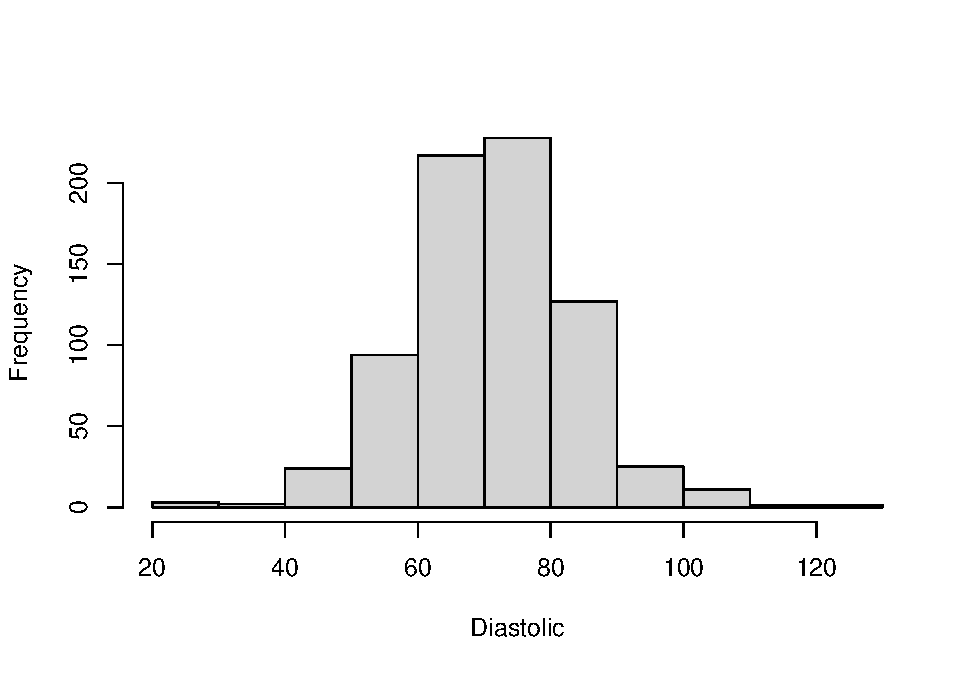
\includegraphics{Repaso_files/figure-latex/unnamed-chunk-6-1.pdf}

\begin{Shaded}
\begin{Highlighting}[]
\FunctionTok{plot}\NormalTok{(}\FunctionTok{density}\NormalTok{(pima}\SpecialCharTok{$}\NormalTok{diastolic,}\AttributeTok{na.rm =}\NormalTok{ T),}\AttributeTok{main =} \StringTok{""}\NormalTok{)}
\end{Highlighting}
\end{Shaded}

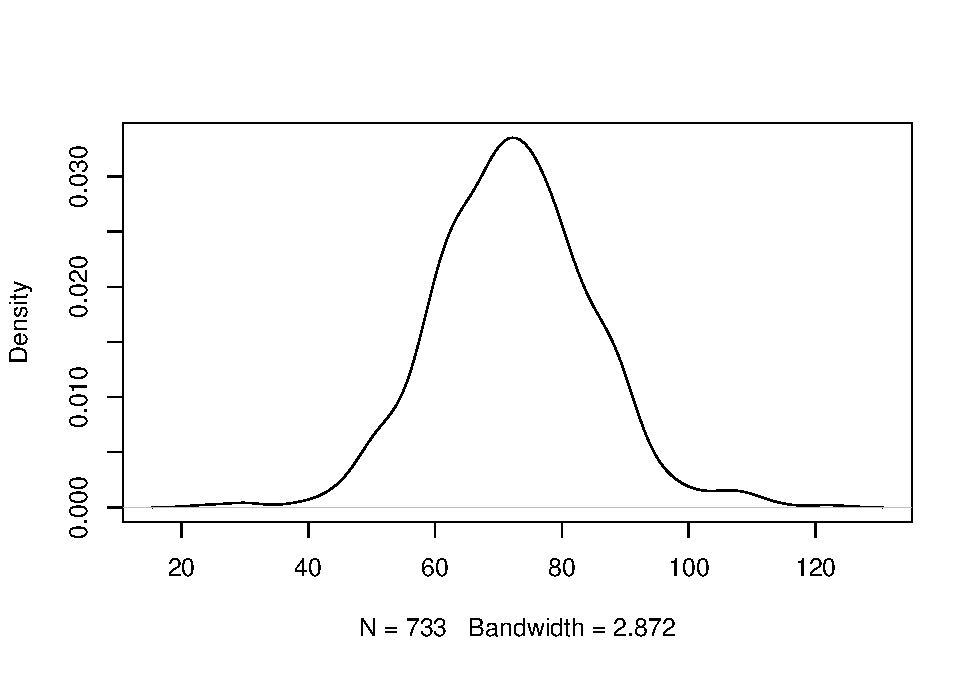
\includegraphics{Repaso_files/figure-latex/unnamed-chunk-6-2.pdf}

\begin{Shaded}
\begin{Highlighting}[]
\FunctionTok{plot}\NormalTok{(}\FunctionTok{sort}\NormalTok{(pima}\SpecialCharTok{$}\NormalTok{diastolic),}\AttributeTok{ylab=}\StringTok{"Sorted Diastolic"}\NormalTok{)}
\end{Highlighting}
\end{Shaded}

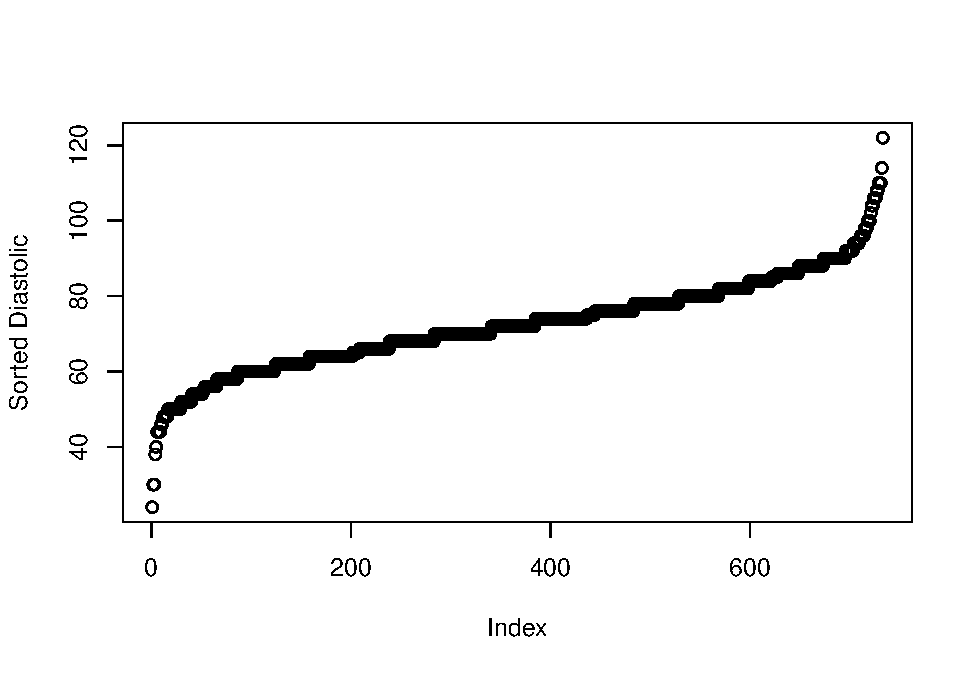
\includegraphics{Repaso_files/figure-latex/unnamed-chunk-6-3.pdf}

\end{document}
